\documentclass[12pt,a4paper]{scrartcl}

\usepackage[a4paper, left=2cm, right=1cm, bottom=1cm, top=1cm, includeheadfoot]{geometry}
\usepackage[ngerman]{babel}
\usepackage[utf8]{inputenc} % comment this if you uncomment utf8x
%\usepackage[utf8x]{inputenc} % uncomment this if there are problems with 'ä', 'ü', 'ö'
\usepackage{ucs}
\usepackage[usenames,dvipsnames]{xcolor}
\usepackage[fleqn]{amsmath}
\usepackage{amsfonts}
\usepackage{amssymb}
\usepackage{color}
\usepackage{listings}
\usepackage{hyperref}
\usepackage{amsfonts}
\usepackage{listings}
\usepackage{scrpage2}
\usepackage{graphicx}


\definecolor{mygray}{rgb}{0.9,0.9,0.9}
\lstset{language=[Visual]Basic, morekeywords={param, local}}


\lstset{
   literate={ö}{{\"o}}1
           {ä}{{\"a}}1
           {ü}{{\"u}}1
           {ß}{{\ss}}1
           {é}{{\'e}}1,
   inputencoding=ansinew,
   extendedchars=true,
   basicstyle=\scriptsize\ttfamily,
   numberstyle=\scriptsize,
   breaklines=true,
   tabsize=2,
   numbersep=5pt
}
\lstdefinestyle{customcpp}{
   language=C++,
   backgroundcolor=\color{mygray},
   numbers=left,
   keywordstyle=\color{blue}\bfseries,
   stringstyle=\color{BrickRed}\ttfamily,
   commentstyle=\color{OliveGreen}\ttfamily,
   showspaces=false,
   showstringspaces=false,
   showtabs=false
}
\lstdefinestyle{customoutput}{
   backgroundcolor=\color{mygray},
   numbers=none,
   showspaces=false,
   showtabs=false
}

\newcommand{\sourceCode}[1]{\lstinputlisting[style=customcpp]{#1}} %beinhaltet alle benötigten Packages etc.
\begin{document}
\graphicspath{{./}}

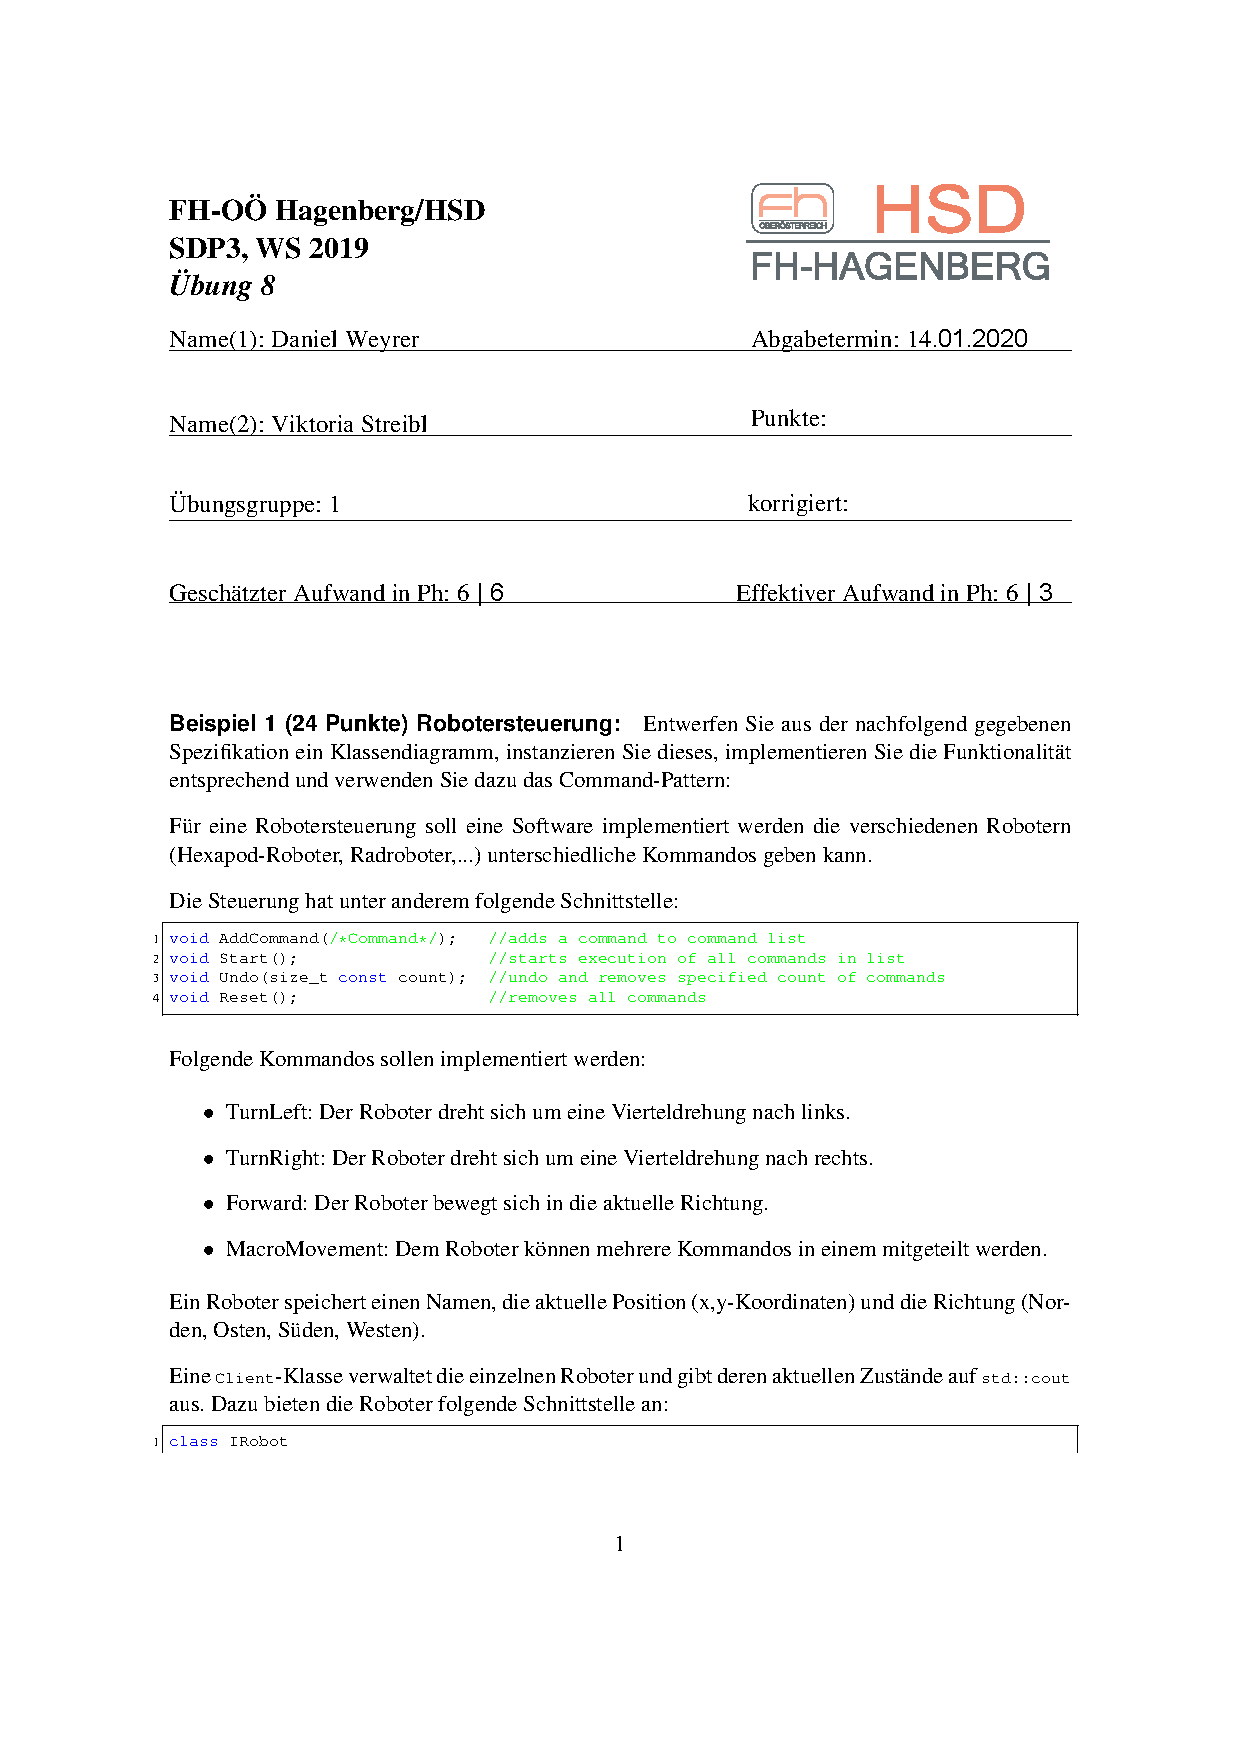
\includepdf[pages=-]{../Angabe.pdf}

\title{SDP - Exercise 08} % Übungsname und Nummer angeben
\subtitle{winter semester 2019/20} % Semester angeben oder auskommentieren, falls nicht erwünscht
\author{
Viktoria Streibl - S1810306013\\
  Daniel Weyrer - S1820306044
} % Autorenname
\date{\today} % Das heutige Datum automatisch einfügen

\maketitle % Titelseite erstellen

\newpage
\tableofcontents % Inhaltsverzeichnis erstellen
\newpage

\ihead{Viktoria Streibl}
\ohead{Daniel Weyrer}
\chead{SDP3-UE Uebung 08}

\section{Organizational}
\subsection{Team}
\begin{itemize}
	\item Viktoria 	Streibl 		- 	S1810306013
	\item Daniel 	Weyrer		-	S1820306044
\end{itemize}

\subsection{Roles and responsibilities}
\subsubsection{Jointly}
\begin{itemize}
	\item Planning
	\item Documentation
	\item Systemdocumentation
	\item Class Diagram
	\item Class FileSystem
	\item TestDriver
\end{itemize}

\subsubsection{Viktoria Streibl}
\begin{itemize}
	\item Visitors
	\subitem Visitor Dump
	\subitem Visitor FilterFiles			
\end{itemize}

\subsubsection{Daniel Weyrer}
\begin{itemize}
	\item Base Class Type
	\item Derived Classes
		\subitem Class File
		\subitem Class Referral
		\subitem Class Folder
	\item Factory
\end{itemize}

\subsection{Effort}

\subsubsection {Viktoria Streibl}
\begin{itemize}
	\item estimated: 12 ph 
	\item actually: 7 ph
\end{itemize}

\subsubsection {Daniel Weyrer}
\begin{itemize}
	\item estimated: 12 ph 
	\item actually: 7 ph
\end{itemize}

\section{Requirenment Definition(System Specification)}

\section{System Design}
\newpage
\subsection{Classdiagram}
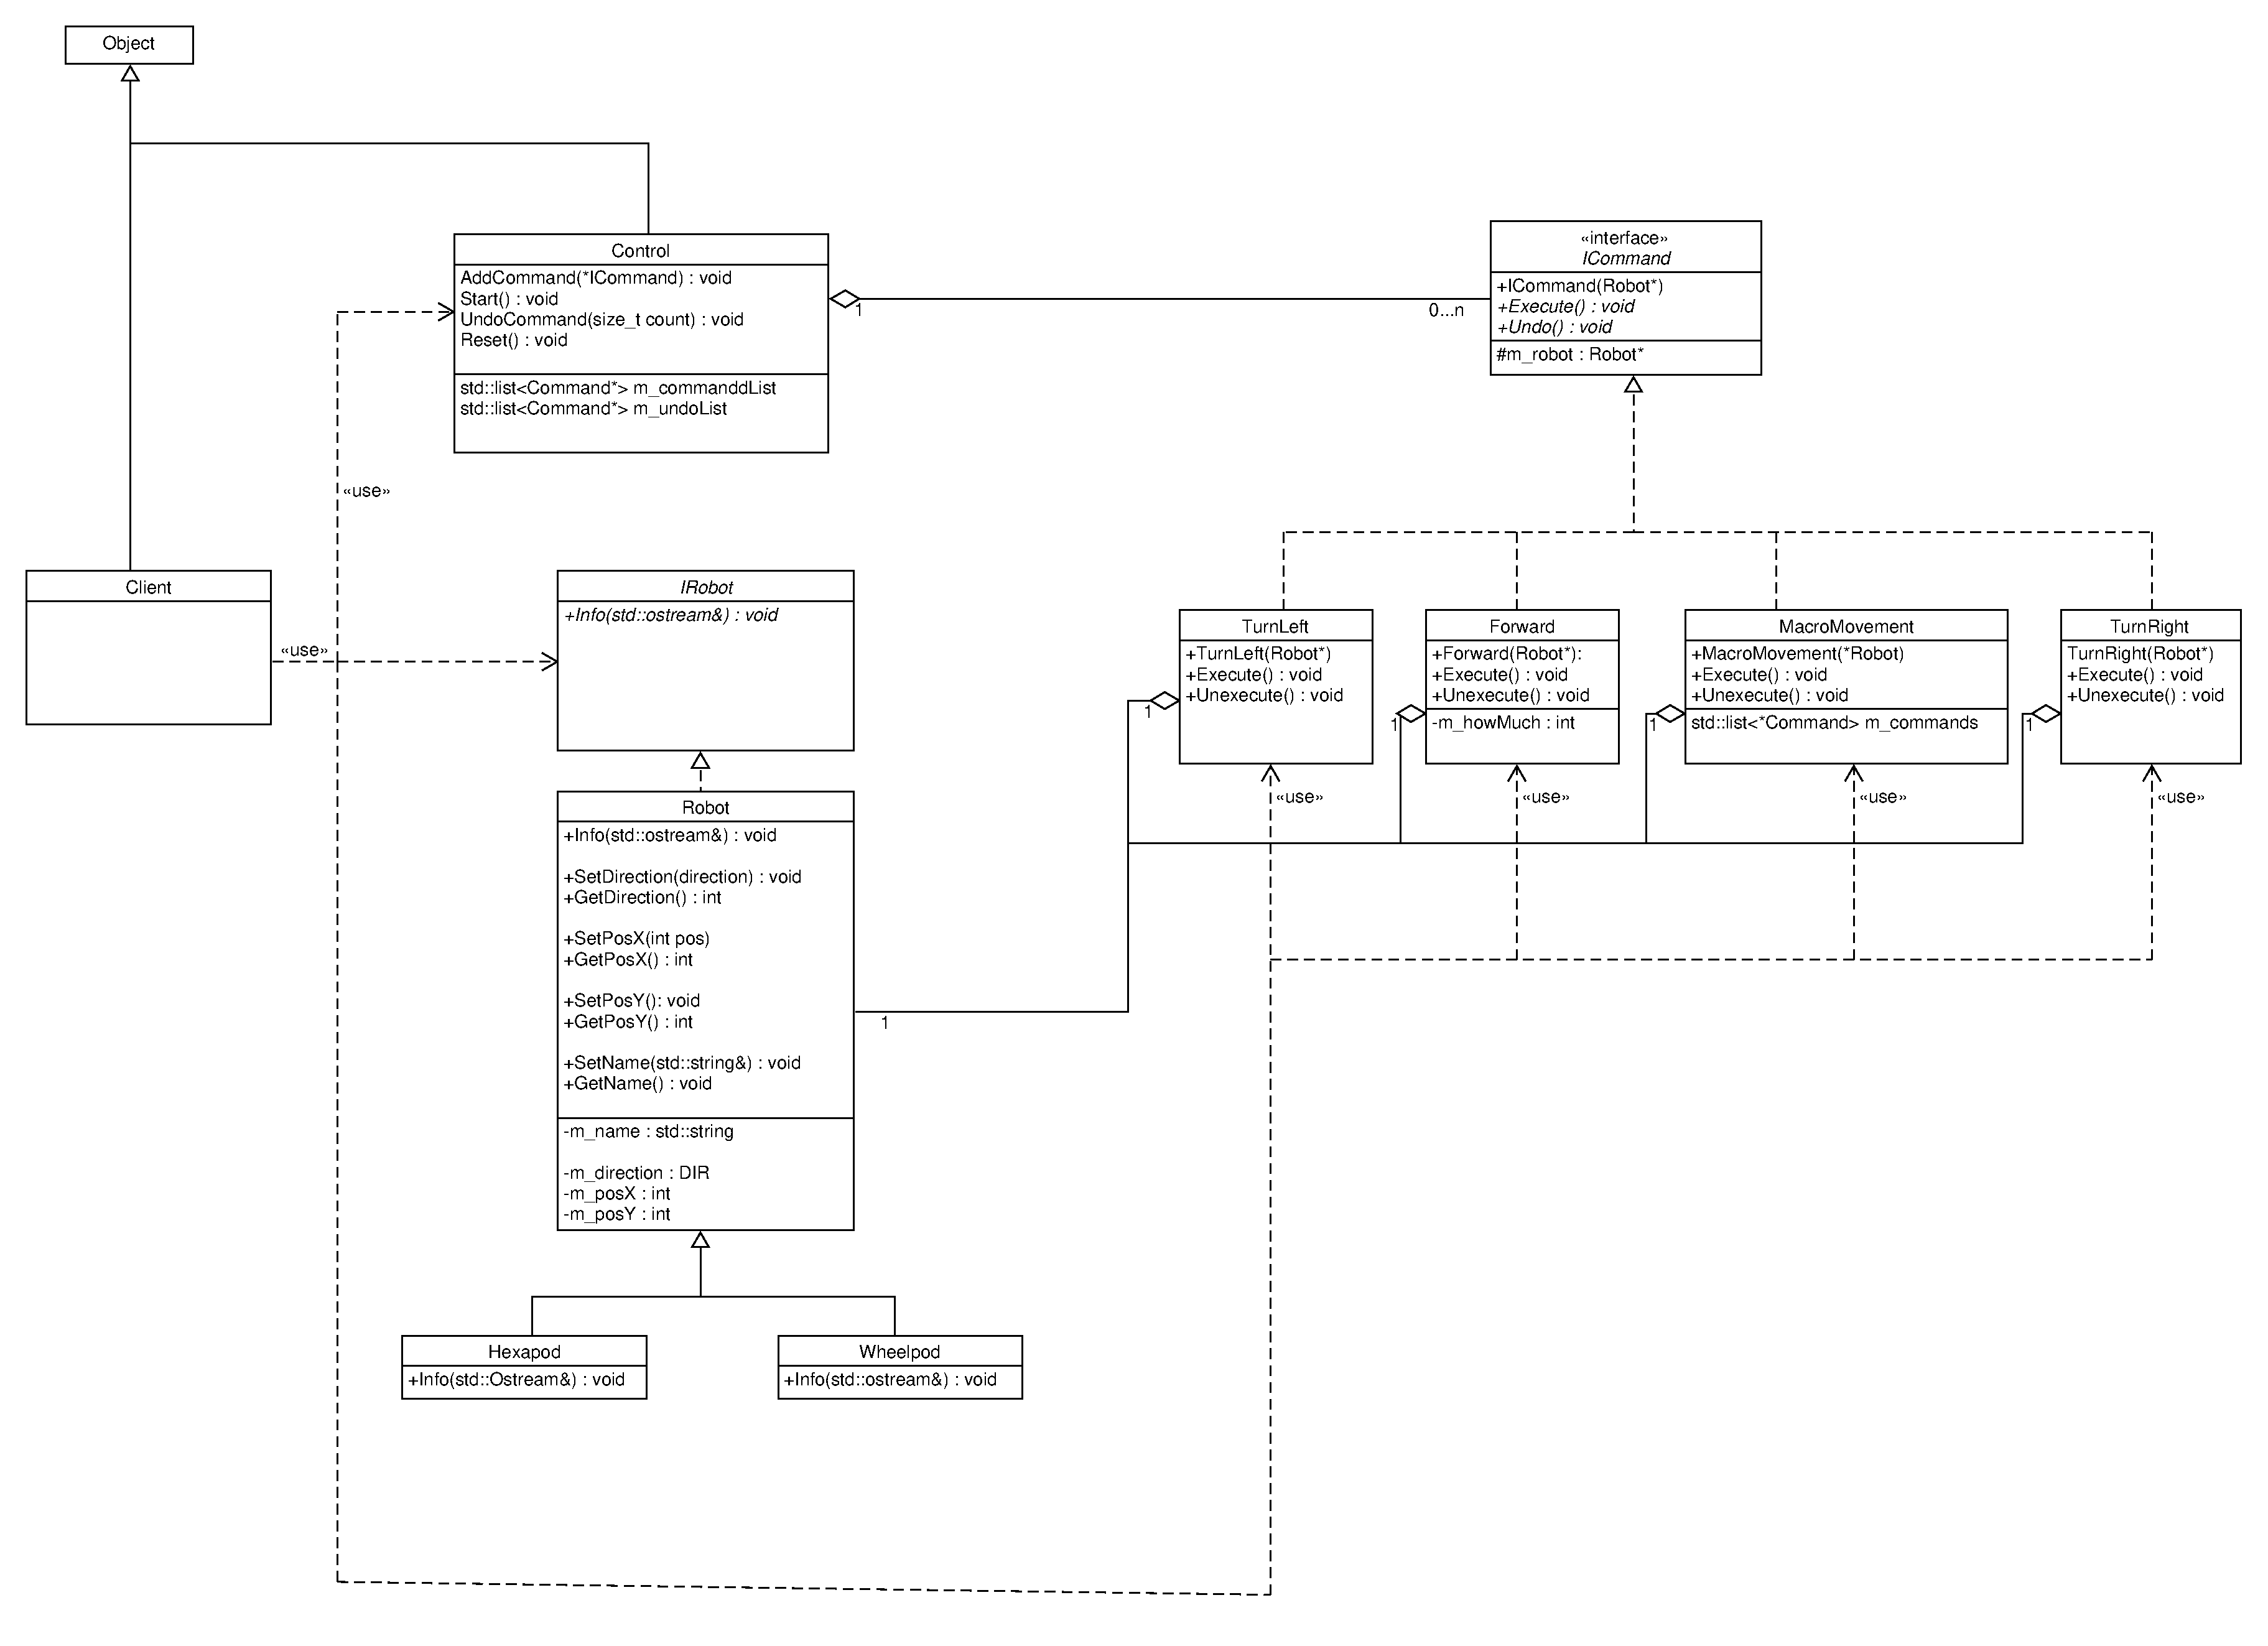
\includegraphics[scale=1, angle=90]{../ClassDiagram.pdf}

\subsection{Design Decisions}
\subsubsection{}



\subsection{TestDriver}
\sourceCode{../../FileSystem/FileSystem/TestDriver.cpp}
\newpage

\section{Source Code}

\subsection{FileSystem}
\subsubsection{FileSystem.h}
\sourceCode{../../FileSystem/FileSystem/FileSystem.h}
\subsubsection{FileSystem.cpp}
\sourceCode{../../FileSystem/FileSystem/FileSystem.cpp}
\newpage

\subsection{Type}
\subsubsection{Type.h}
\sourceCode{../../FileSystem/FileSystem/Type.h}
\subsubsection{Type.cpp}
\sourceCode{../../FileSystem/FileSystem/Type.cpp}
\newpage

\subsection{File}
\subsubsection{File.h}
\sourceCode{../../FileSystem/FileSystem/File.h}
\subsubsection{File.cpp}
\sourceCode{../../FileSystem/FileSystem/File.cpp}
\newpage

\subsection{Referral}
\subsubsection{Referral.h}
\sourceCode{../../FileSystem/FileSystem/Referral.h}
\subsubsection{Referral.cpp}
\sourceCode{../../FileSystem/FileSystem/Referral.cpp}
\newpage

\subsection{Folder}
\subsubsection{Folder.h}
\sourceCode{../../FileSystem/FileSystem/Folder.h}
\subsubsection{Folder.cpp}
\sourceCode{../../FileSystem/FileSystem/Folder.cpp}
\newpage

\subsection{IVisitor}
\subsubsection{IVisitor.h}
\sourceCode{../../FileSystem/FileSystem/IVisitor.h}

\subsection{Dump}
\subsubsection{Dump.h}
\sourceCode{../../FileSystem/FileSystem/Dump.h}
\subsubsection{Dump.cpp}
\sourceCode{../../FileSystem/FileSystem/File.cpp}
\newpage

\subsection{FilterFiles}
\subsubsection{FilterFiles.h}
\sourceCode{../../FileSystem/FileSystem/FilterFiles.h}
\subsubsection{FilterFiles.cpp}
\sourceCode{../../FileSystem/FileSystem/FilterFiles.cpp}
\newpage

\subsection{Factory}
\subsubsection{Factory.h}
\sourceCode{../../FileSystem/FileSystem/Factory.h}
\subsubsection{Factory.cpp}
\sourceCode{../../FileSystem/FileSystem/Factory.cpp}
\newpage

\subsection{TestDriver}
\subsubsection{TestDriver.cpp}
\sourceCode{../../FileSystem/FileSystem/TestDriver.cpp}
\newpage


\end{document}